% Going off the Thesis guidelines available here: http://www.lboro.ac.uk/students/welcome/research/codes-of-practice/appendices/
% A4 paper size selected, default is 11pt font, to change to 12pt use [a4paper, 12pt] as option to documentclass
\documentclass[a4paper]{report}

% Some useful packages for including images, colored font, etc.
\usepackage[dvips]{graphicx}
\graphicspath{{Figures/}}

\makeatletter
\def\maxwidth{\ifdim\Gin@nat@width>\linewidth\linewidth\else\Gin@nat@width\fi}
\def\maxheight{\ifdim\Gin@nat@height>\textheight\textheight\else\Gin@nat@height\fi}
\makeatother
\setkeys{Gin}{width=\maxwidth,height=\maxheight,keepaspectratio}
\usepackage{amssymb,amsmath}
\usepackage{longtable}
\usepackage{booktabs}

\usepackage{listings}
\usepackage{xcolor}
 
\definecolor{codegreen}{rgb}{0,0.6,0}
\definecolor{codegray}{rgb}{0.5,0.5,0.5}
\definecolor{codepurple}{rgb}{0.58,0,0.82}
\definecolor{backcolour}{rgb}{0.95,0.95,0.92}
 
\lstdefinestyle{mystyle}{
    backgroundcolor=\color{backcolour},   
    commentstyle=\color{codegreen},
    keywordstyle=\color{magenta},
    numberstyle=\tiny\color{codegray},
    stringstyle=\color{codepurple},
    basicstyle=\ttfamily\footnotesize,
    breakatwhitespace=false,         
    breaklines=true,                 
    captionpos=b,                    
    keepspaces=true,                 
    numbers=left,                    
    numbersep=5pt,                  
    showspaces=false,                
    showstringspaces=false,
    showtabs=false,                  
    tabsize=2
}
 
\lstset{style=mystyle}

\usepackage[numbers]{natbib}

\usepackage{color}
\usepackage{url}
% Used for subfigures
\usepackage{subcaption}
% Used for landscape pages
\usepackage{pdflscape}
% Used for hyper-links in contents, etc.
\usepackage[hidelinks]{hyperref}
\hypersetup{
    linktoc=all
}

% Global bibliography style
\bibliographystyle{unsrt}

% Set margins in all document to 3.5cm as per guidelines for binding
\usepackage[includeheadfoot,margin=3.5cm]{geometry}

% Used to including pdf files within pages
% use [draft] as option to output empty spaces rather than rendering all pages (useful when including lots of pdfs)
\usepackage{pdfpages}

% Used to produce headers and footers
\usepackage{fancyhdr}
\pagestyle{fancyplain}

% Used for removing title in bibliography sections
\usepackage{titlesec}

% Used to generate lists of abbreviations
\usepackage{nomencl}
\makenomenclature 
\renewcommand{\nomname}{List of Abbreviations} 

% To have a separate bibliography per Chapter uncomment this line
% See Introduction/Introduction.tex for example how to include the bibliography
%\usepackage{chapterbib}

% Line spacing defined at 1 and a half. I know it says 1.3 but its 1 and a half.
\linespread{1.3}

% Setup headers and footers
\fancyhf{}
\lhead{\leftmark}
% Center on all pages
% \fancyhead[C]{---Draft---}
% Page number placed on right side on odd pages and left side on even pages
\fancyfoot[RO, LE] {\thepage}


\begin{document}

% Give \subsubsection numbers
\setcounter{secnumdepth}{4}

% Title, Author, Abstract, Acknowledgement, Table of Content, List of Figures, List of Tables and List of Abbreviations
% Front matter of the Thesis
% Title page
% Loughborough University Thesis Access Form
% Loughborough University Certificate of Originality
% Abstract
% Acknowledgements
\title{\bf Vehicle Make \& Model Recognition}

\author{by\\Zhihao DAI\\
\\
{\bf COP507 Computer Vision \& Embedded Systems}\\
{\bf Coursework Report}\\
\\
Loughborough University\\
\\
\copyright
\hspace{1 dd} Zhihao DAI 2020\\
\\
Jan. 2020
}
\date{} % Used to remove date from title so it can be set at any date rather than the current date

\maketitle

% Set page numbers to roman numerals for front matter
\pagenumbering{roman}

% % PDF exports of Word Documents available (Exported August 2012)
% % Thesis Access Form
% \includepdf[pages=1, pagecommand=, templatesize={5in}{10in}]{Front/LU/access.pdf}
% % Certificate of Originality
% \includepdf[pages=-, pagecommand=, templatesize={5in}{10in}]{Front/LU/origin.pdf}

% Abstract
\addcontentsline{toc}{chapter}{Abstract}
\chapter*{Abstract}
In this paper, a general architecture of Vehicle Make \& Model Recognition (VMMR) system is designed and implemented.
A variety of features extraction methods, dimensionality reduction methods, classification methods are evaluated and compared.
The best performance is achieved when Square Mapped Gradients (SMG) is used for feature extraction, Principal Component Analysis (PCA) ($\sigma = 70$) for dimensionality reduction and Support Vector Machine (SVM) for classification.
The best accuracy score is $99.62\%$, precision $99.77\%$, recall $99.62\%$ and F1-score $99.70\%$.

% % Acknowledgements
% \addcontentsline{toc}{chapter}{Acknowledgements}
% \chapter*{Acknowledgements}
% Acknowledgement section.

% Set the depth for your table of content
% Currently set at 2 (Chapter, Section, Subsection)
\setcounter{tocdepth}{2}
% Include a table of content
\tableofcontents

% Include a list of figures
\addcontentsline{toc}{chapter}{List of Figures}
\listoffigures

% Include a list of tables
\addcontentsline{toc}{chapter}{List of Tables}
\listoftables

% Include a list of Listings
\addcontentsline{toc}{chapter}{List of Listings}
\renewcommand*{\lstlistlistingname}{List of Listings}
\lstlistoflistings

% Include a list of abbreviations using nomenclature package
%\addcontentsline{toc}{chapter}{List of Abbreviations}
%\printnomenclature[3cm] 

\newpage

% Set page numbering to arabic for body of Thesis
\pagenumbering{arabic}


% To keep everything neat I included each chapter as a separate .tex file
% Each contains a single chapter, they include all the settings defined in this .tex file
% Allows easier moving around of chapters

% Use \include{<path to .tex file>} to include documents
% For example
\chapter{Introduction}
\label{chap:introduction}

Automatic Number Plate Recognition (ANPR) systems are widely used for policing, traffic monitoring and access control.
They have proven to be accurate and efficient under most scenarios.
However, ANPR systems are vulnerable to plate cloning, forgery or erosion.


A Vehicle Make \& Model Recognition (VMMR) system receives an image of a vehicle as input and outputs the make and model of that vehicle.
Such system could strengthen the security of existing ANPR systems by providing a matching between vehicle types and number plates.
For example, in access control, if the number plate is not registered under the detected vehicle type, a security warning is raised and manual intervention is required.

In this paper, we design and implement a VMMR system. The input to the system is a cropped frontal image of a vehicle and the output is the make and model of the vehicle.




\section{Related Work}

Due to the significance of VMMR systems, many approaches have been proposed for building VMMR systems in recent years. 
% Analysis of Features for Rigid Structure Vehicle Type Recognition.
Petrovic and Cootes \citep{petrovic2004analysis} extracted simple features such as Sobel Edge Response, Edge Orientation, Square Mapped Gradients from images in the database. 
Features are then represented and stored either in full dimension or in low dimension through Principal Component Analysis (PCA).
Given a new image, the VMMR system predicts the vehicle type by finding the closest match in dot product distance.
Their experiments on a dataset of $1132$ frontal images of $77$ vehicle classes showed that direct matching by Square Mapped Gradients features achieved the lowest vertification error of $3.5\%$.

% Car Make and Model Recognition Combining Global and Local Cues.
AbdelMaseeh et al. \citep{abdelmaseeh2012car} observed that unlike most object recognition tasks, VMMR poses a challenge of distingushing between similar classes under the same category (ie. vehicle).
Based on this observation, they proposed the combination of global and local descriptors for VMMR.
While global shape descriptors capture differences across categories, local shape and appearance descriptors for segmented regions capture inter-class varieties.
An image is matched to the class with the smallest weighted sum of global and local dissimilarity measures.

% Automatic Make and Model Recognition from Frontal Images of Cars.
Pearce and Pears \citep{pearce2011automatic} suggested using Harris corner detectors \citep{harris1988combined} for features extraction and either K-Nearest Neighbour (KNN) or Naive Bayes Classifier for classification in VMMR systems.
Local Harris strengths are computed through recursively dividing the image into quadrants and computing the sum of Harris corner response for each quadrant.
Such features are then normalised through being devided by the sum of higher level strengths.
For an input image of 150 by 150, a feature vector of Locally Normalised Harris Strengths (LNHS) of depth 5 is retrived and only one-twentieth the size of the original Harris corner response.
Their experiments on a dataset of $262$ frontal images of $74$ vehicle classes showed that LNHS with Naive Bayes Classifier achieved the highest accuracy of $96\%$. 
Using LNHS as features speeds up the training of a classifier and does not reduce the accuracy.


% Real-Time Vehicle Make and Model Recognition Based on a Bag of SURF Features.
Siddiqui et al. \citep{siddiqui2016real} proposed using Speeded Up Robust Features (SURF) \citep{bay2006surf} for features extraction and Support Vector Machines (SVM) for classification.
Following Sivic and Zisserman's work on Bag-of-Features method \citep{sivic2003video}, a dictionary (bag) of SURF features was constructed using K-Means clustering algorithm.
An image can be then transformed into a fixed-length vector of visual words occurances and be fed into a SVM classifier for vehicle type recognition.
High accuracy score of $94.84\%$ was obtained on a large dataset of $6601$ frontal images of $29$ vehicle classes.


% Two Dimensional Statistical Linear Discriminant Analysis for RealTime Robust Vehicle Type Recognition.
Zafar et al. \citep{zafar2007two} observed that dimensionality reduction methods used in many VMMR systems such as Principal Component Analysis (PCA) enhances the inner-class variance and can lead to miss-classification.
In their setting, the raw pixel values of the image is directly projected to low-dimension space through Two Dimensional Linear Discriminant Analysis (2D-LDA) \citep{li20052d}.
A match is found by minmizing the Euclidean distance to those in the training images set.
The usage of 2D-LDA instead of PCA solves the variance problem by maximizing the ratio of intra-class variance to the inter-class variance.
An accuracy score of $91\%$ was obtained on a dataset of $271$ frontal images of $25$ vehicle classes ($8$ images per class for training and the rest for validation).

% Localised Contourlet Features in Vehicle Make and Model Recognition.
Zafar et al. \citep{zafar2009localized} later proposed using localized Contourlet transform for features extraction, 2D-LDA for dimensionality reduction, and SVM for classification.
They reported a boosted accuracy of $96\%$ on the same frontal car images dataset in \citep{zafar2007two}.


% Mid-Level-Representation based Lexicon for Vehicle Make and Model Recognition.
Fraz et al. \citep{fraz2014mid} introduced an innovative framework of Mid-Level-Representation of densely sampled features into VMMR.
The framework starts by extracting patches around key-points detected by Difference of Gaussians (DoG) detector.
For each extracted patch, A set of Scale-Invariant Feature Transform (SIFT) \citep{lowe2004distinctive} feature descriptors are computed and reduced dimensionality by PCA.
Fisher Vector \citep{jaakkola1999exploiting}, a Mid-Level-Representation (MLR), for the patch is then generated based on Gaussian Mixture Model (GMM), following Perronnin et al.'s work \citep{perronnin2010improving}.
Fisher Vector for patches in images within the same class are visual words and collectively form a sub-lexicon.
A lexicon of the training set images is essentially a collection sub-lexicons of all classes.
Given a new image, the VMMR system 
extracts patches from the image, 
assigns each patch to a visual word by Euclidean distance within each sub-lexicon, 
classifies the image to the class (sub-lexicon) with the highest sum of similarity score of the word-patch matches.
Fraz et al. reported an accuracy of $97.60\%$ on the dataset used in \citep{zafar2009localized} and $84.31\%$ on a new dataset. The new dataset, coined 'Loughborough Cars (LC) Dataset', is composed of $1537$ frontal images of $75$ vehicle classes.


\section{Dataset}
\label{sec:dataset}
There is a diverse set of datasets for VMMR task and Tafazzoli et al. \citep{tafazzoli2017large} presented a thorough survey of them.
Our proposed system is trained and evaluated on a superset of the dataset in \citep{zafar2007two,zafar2009localized,fraz2014mid} of $530$ frontal images from $27$ vehicle make and model classes.
For each class, $6$ images are used for training and the rest for validation.
Both the training set and validation set are pre-processed to extract Regions of Interest (ROI). See Section \ref{sec:pre-processing} for more details.

\begin{figure}
\centering
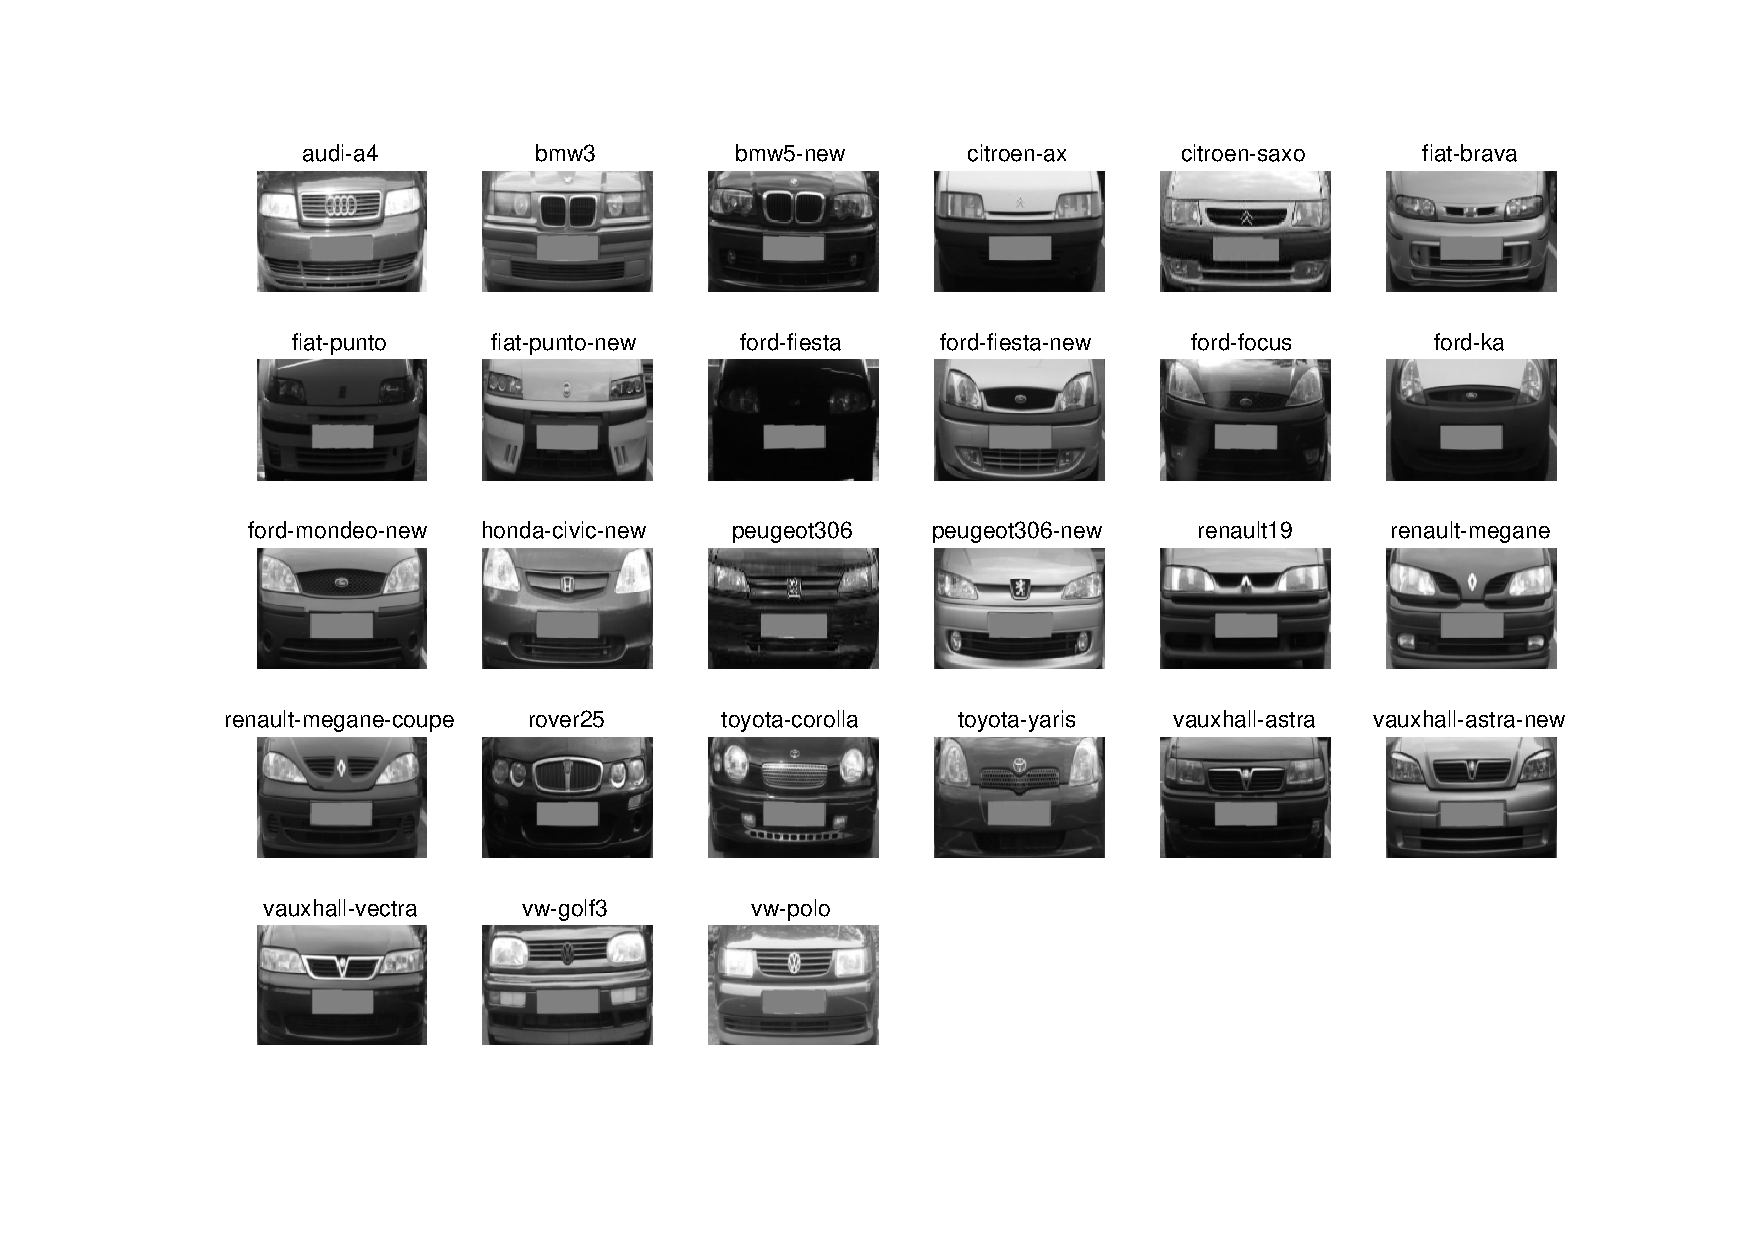
\includegraphics{classes}
\caption{Samples of All $27$ Vehicle Make and Model Classes in the Dataset.}
\label{fig:classes}
\end{figure}

\section{Comparison to Our Method}

In this paper, we make use of 
Raw Image Pixels, Sobel Edge Response and Square Mapped Gradients following Petrovic and Cootes's \citep{petrovic2004analysis} work, 
Locally Normalised Harris Strengths (LNHS) from Pearce and Pears's work \citep{pearce2011automatic}, and 
Bag of Speeded Up Robust Features (SURF) from Siddiqui et al.'s work \citep{siddiqui2016real} 
interchangeably in our features extraction module.
We use Principal Component Analysis (PCA) for optional dimensionality reduction module and either 
K-Nearest Neighbour (KNN) or
Support Vector Machine (SVM) for classification module.

Despite having a smaller number of $6$ training images per vehicle class compared to $8$ in Zafar et al.'s work \citep{zafar2007two} and $10$ in Zafar et al.'s work \citep{zafar2009localized} and simplicity of features computation compared to Mid-Level-Representation in Fraz et al.'s work \citep{fraz2014mid}, our method achieves a higher accuracy score of $98\%$ on the validation set.







\chapter{System Design}
\label{chap:design}

\section{Assumptions}

% \section{Graphical User Interface}

\section{Feature Extraction Methods}

\section{Dimension Reduction Methods}

\section{Classification Methods}




\chapter{Experiments and Results}
\label{chap:experiments}

Environment, etc.

\section{Pre-processing}
\label{sec:pre-processing}

\section{Cross-Validation}

\section{Merits of Performance}

\section{Effects of Features Extraction Methods}
\label{sec:effects-fe}

\section{Effects of Dimensionality Reduction Methods}
\label{sec:effects-dim}

\section{Effects of Classification Methods}
\label{sec:effects-cls}


\chapter{Convolution Neural Network Model}
\label{chap:cnn}

\section{Architecture}
For VMMR tasks, a simple Convolution Neural Network (CNN) model is also considered, as presented in \ref{fig:cnn}.

\begin{figure}
\centering
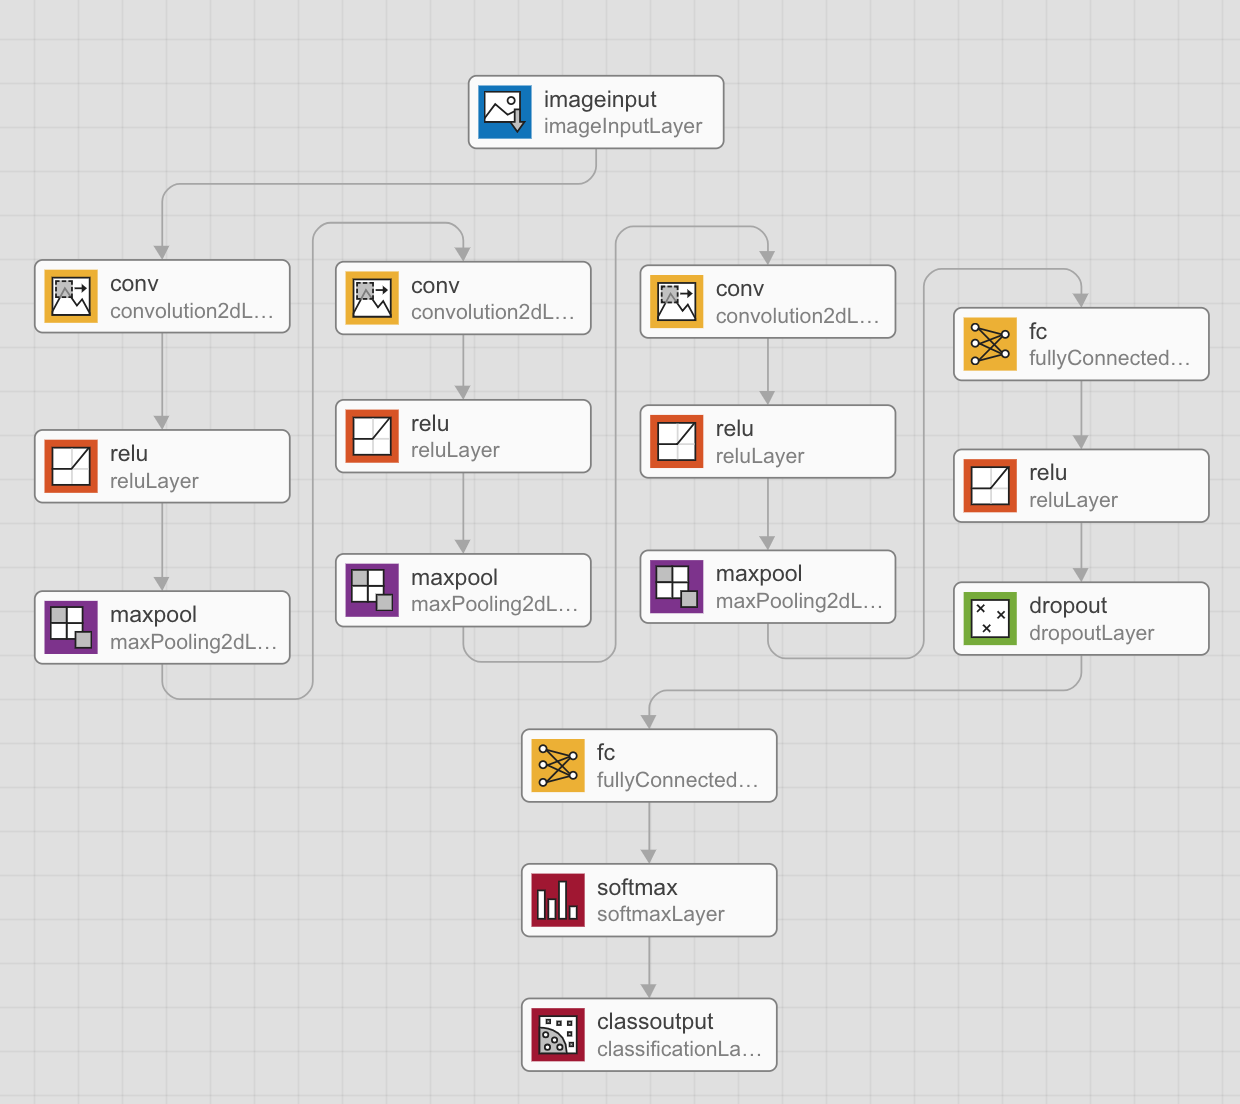
\includegraphics{cnn}
\caption{Architecture of Our Proposed CNN.}
\label{fig:cnn}
\end{figure}

The input image of size $(140, 140, 1)$ is fed into the first convolution layer and activated by a ReLU function. The convolution layer has $32$ filters of $(5, 5)$, stride of $2$ and produces an output of $(70, 70, 32)$.
The layer picks up simple features such as edges, colours, curves from the image.
It is followed by a max pooling layer with filter size of $(3, 3)$ and stride of $2$ to reduce dimensionality. The output has a size of $(35, 35, 32)$ and is fed into the second convolution layer.

The second convolution layer has $32$ filters of $(3, 3)$, stride of $2$ and produces an output of $(18, 18, 32)$. 
The layer picks up more specific features such as squares, circles and triangles from the image.
It is activated by a ReLU function and followed by a max pooling layer with filter size of $(3, 3)$ and stride of $2$ to reduce dimensionality. The output has a size of $(9, 9, 32)$ and is fed into the third convolution layer.

The third convolution layer also has $32$ filters of $(3, 3)$, stride of $1$ and produces an output of $(9, 9, 32)$. 
This layer picks up high-level features such as headlights, front beams, logos from the image.
It is activated by a ReLU function and followed by a max pooling layer with filter size of $(3, 3)$ and stride of $2$ to reduce dimensionality. The output has a size of $(5, 5, 32)$ and is fed into the first fully connected layer.

The first fully connected layer has $256$ hidden units and is activated by a ReLU function. This layer introduces more complexity into the network and allows high-level features located at different locations in the image to be combined.
It is followed by a dropout layer with rate of $0.5$, which introduces regularization into the model and prevents over-fitting.
The output is fed into the second fully connected layer.

The first fully connected layer has $27$ hidden units, the same size as the number of vehicle classes, and is activated by a Softmax function for the final classification output.


\section{Overfitting Issues}
Our proposed CNN model has $213,467$ parameters, much larger to other machine learning models used previously. Thus, the model is prune to overfitting.
The following strategies can be adopted to prevent overfitting in the model.

\begin{enumerate}
\item
	Introduce a regularization term into the loss function. That is, the new loss function $L_{new}(W) = L(W) + \lambda R(W)$, where $R(W)$ is a regularization term for the weights $W$. Typically, $R(W) = W^2$ and it forces the network to make full use of the inputs at each layer.
\item
	Introduce a dropout layer in between different layers. The dropout layer randomly drops a percentage of its input, thus forcing the next layer to not rely on a small set of its inputs.
\item
	Early stopping. When the model is being trained on the dataset, the decrease in loss on the training set and the increase in loss on the validation set is a sign of overfitting. In such cases, the model should be stopped training to prevent further overfitting.
\end{enumerate}

\section{Insufficient Dataset}
Given the small size of our dataset ($530$ images in total), the average number of parameters per image is $403$. 
Such amount of paramters signal that the size of our dataset is insufficient.
In the case that time and resouces are limited for collecting new data, several alternative solutions could be considered.

\begin{enumerate}
\item
	Apply data augmentation to the dataset to generate more images for training. The operations for data augmentation include rotation, scaling, shearing and translation.
\item
	Use pre-trained CNN models such as AlexNet\citep{krizhevsky2012imagenet}, GoogLeNet\cite{szegedy2015going} and ResNet\citep{he2016deep} in a transfer learning scheme. Since our dataset is small, it is difficult to fine-tune the whole network. Therefore, only the last few layers of pre-trained CNN networks are replaced and re-trained.
\end{enumerate}


% \section{Performance}







\chapter{Discussion}
\label{chap:discussion}

\section{Conclusions}

\section{Future Work}



% Include a Chapter names References to the table of content
\addcontentsline{toc}{chapter}{References}
% Rename Bibliography to References
\renewcommand\bibname{References}
\bibliography{Bib/tex}

% Include authors publications and appendix section
% \include{Publications/Publications}
% Appedix
\appendix

\begingroup

\chapter{Source Code}
\label{app:code}



\endgroup


\end{document}
